\documentclass{article}

\usepackage{minted}
\usepackage[most]{tcolorbox}
\usepackage{geometry}
\usepackage{enumitem}
\usepackage{hyperref}
\usepackage{hyperref}
\usepackage[parfill]{parskip}
\usepackage{wrapfig}
\usepackage{accsupp}

\geometry{margin=0.8in}
\definecolor{lightgreen}{rgb}{0.56, 0.93, 0.56}
\definecolor{moonstoneblue}{rgb}{0.45, 0.66, 0.76}
\definecolor{magenta}{rgb}{0.8,0.66,0.76}
\begin{document}
\BeginAccSupp{}
\begin{flushright}
Computational Biology ~\\
Tufts University Bio 35 ~\\
Fall 2021 ~\\ ~\\
\end{flushright}
\begin{center}{\textbf{\Large{Spotlight 5: Shane Campbell-Staton}}}\end{center}

\textit{Please note that in general I have taken/adapted the words of our Spotlight subjects from their own websites to describe their work. I have done this in an effort to maintain accuracy in describing their research programs. Please do not copy paste text from their papers/websites in your assignments!}

\begin{wrapfigure}{L}{0.14\textwidth}
\begin{center}
 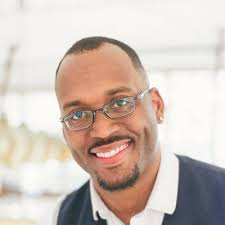
\includegraphics[width=0.13\textwidth]{images/shane-campbell-staton.jpeg}
 \end{center}
\end{wrapfigure}
~\\ As part of our unit on natural selection and population genetics, we are going to explore the work of Shane Cambell-Staton. Prof. Campbell-Staton's lab studies how climate shapes demographic history and adaptation over prehistoric and contemporary time periods. He combines comparative physiology, genomics, field experimentation and environmental niche modeling to understand how novel environments produce phenotypic and genetic differences between lineages. A major goal of his research is to understand how complex phenotypes respond to anthropogenic climate change. Dr. Campbell-Staton is a faculty member at UCLA.
~\\ 

Please read the following articles about Prof. Campbell-Staton's work: 
\begin{enumerate}
\item \texttt{\href{https://science.sciencemag.org/content/357/6350/451.full}{https://science.sciencemag.org/content/357/6350/451.full}}
\item \texttt{\href{https://www.theatlantic.com/magazine/archive/2018/10/up-all-night/568291/}{https://www.theatlantic.com/magazine/archive/2018/10/up-all-night/568291/}}
\end{enumerate}

And listen to the following podcast about Prof. Campbell-Staton's work:
\begin{enumerate}
\item \texttt{\href{https://www.scientificamerican.com/podcast/episode/cold-snap-shapes-lizard-survivors/}{https://www.scientificamerican.com/podcast/episode/cold-snap-shapes-lizard-survivors/}}
\end{enumerate}

\subsubsection*{Written Assignment} 
After reading about Prof. Campbell-Staton please write a reflection (max one page) on what you discovered. You might wish to address some of the following: 

\begin{enumerate}
\item What was most interesting to you in reviewing these resources?
\item What did you learn from these resources about rapid adaptation in natural populations and the role of climate and/or human activity? How can computational tools help us understand how rapid adaptation works?
\item What new questions do you have after reviewing these resources?
\item What do these resources tell you about the types of people that do computational biology, or their motivations?
\end{enumerate}

\EndAccSupp{}
\end{document}